% D04-003. AI-01 P0043--P0057, P0095--P0109.
\section{Общая методика оценки моделей}
\label{sec:ch4_evaluation_methodology}

При анализе осциллограмм большая часть отсчётов относится
к установившемуся режиму. Аварийные события занимают сравнительно
небольшую часть записи. Поэтому общая доля правильных ответов
не даёт достаточного представления о качестве модели.
Алгоритм, который всегда сообщает об отсутствии повреждения,
может правильно описывать большую часть времени и при этом
пропускать все интересующие события. Для оценки распознавания
используются показатели правильного обнаружения, пропусков
и ложных положительных решений. Эта методика применяется
далее при сравнении архитектур и представлений сигналов,
а также при проверке нейросетевого РНМ.

\subsection{Правильные решения и ошибки распознавания}
\label{sec:ch4_metric_decisions}

Для выбранного события положительной считается метка его
наличия, отрицательной метка отсутствия. Обозначение $TP$
соответствует числу случаев, когда событие присутствовало
и было обнаружено. $FN$ обозначает пропущенные положительные
примеры, $FP$ ложные сообщения о событии, а $TN$ правильные
решения об его отсутствии. На рисунке~\ref{fig:ch4_metric_errors}
показано соотношение этих четырёх групп. Круг выделяет примеры,
которые модель отнесла к положительному классу.

\begin{figure}[htbp]
    \centering
    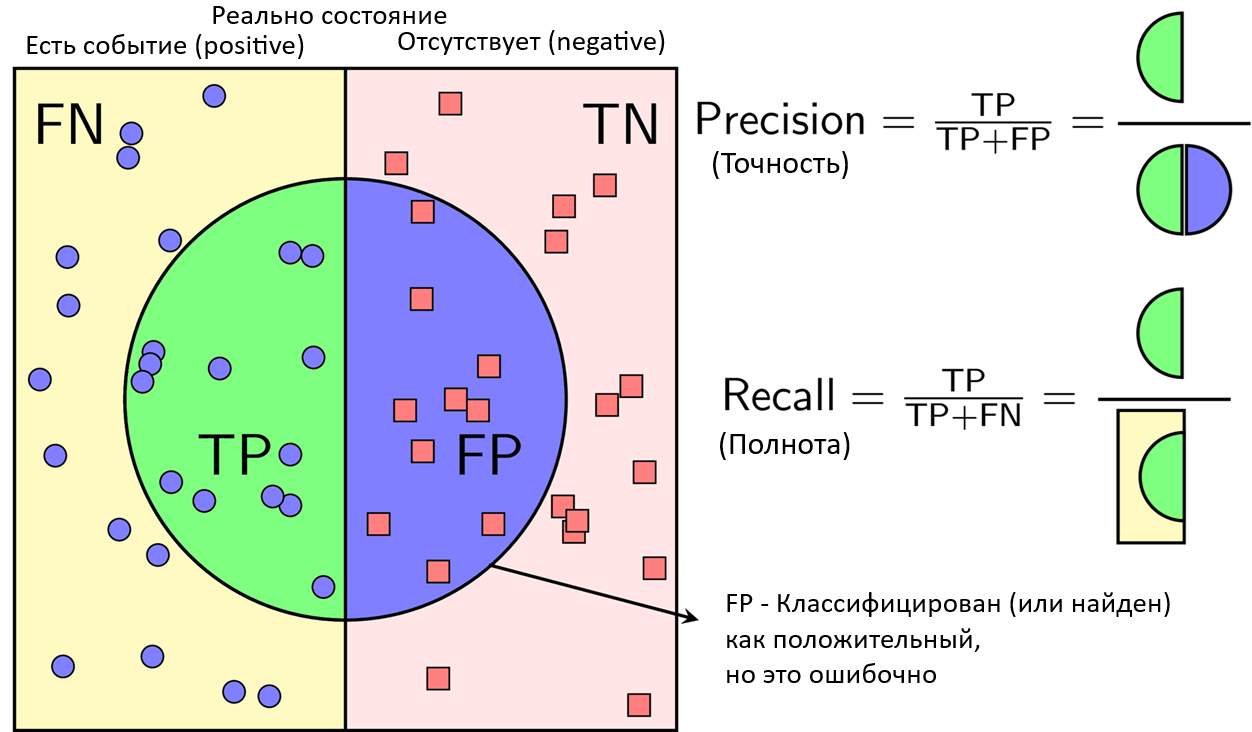
\includegraphics[width=0.95\textwidth]{ml_metric_errors.png}
    \caption{Правильные решения и ошибки при распознавании события.
    Иллюстрация из исследования архитектур нейросетей}
    \label{fig:ch4_metric_errors}
\end{figure}

Точность положительных решений Precision показывает, какая
часть сообщений модели о событии соответствует целевой разметке.
Полнота Recall показывает, какая часть размеченных положительных
примеров была обнаружена. Их гармоническое среднее F1 уменьшает
итоговую оценку при недостаточности любого из двух показателей.
Эти величины определяются выражениями
\begin{equation}
    \mathrm{Precision}=\frac{TP}{TP+FP},\qquad
    \mathrm{Recall}=\frac{TP}{TP+FN},\qquad
    F_1=\frac{2TP}{2TP+FP+FN}.
    \label{eq:ch4_classification_metrics}
\end{equation}
Если знаменатель равен нулю, соответствующая оценка по этой
формуле не определена.

В задачах РЗА пропуск повреждения и ложное сообщение имеют
разные последствия. Полнота характеризует обнаружение событий
в пределах принятой разметки, а Precision позволяет оценивать
долю ложных сообщений среди положительных решений.
При проверке измерительного органа рассматриваются
конкретные режимы, уставки и допустимые области действия.
Поэтому сами показатели классификации не заменяют проверку
чувствительности и селективности защиты.

\subsection{Порог решения и ROC-AUC}

Нейросеть сначала формирует числовую оценку. Положительное
решение получается после сравнения её с выбранным порогом.
Изменение порога меняет соотношение обнаруженных событий
и ложных положительных решений. ROC-кривая показывает эту
зависимость по доле обнаруженных положительных примеров
и доле ложных решений среди отрицательных примеров
\begin{equation}
    \mathrm{TPR}=\frac{TP}{TP+FN},\qquad
    \mathrm{FPR}=\frac{FP}{FP+TN}.
    \label{eq:ch4_roc_rates}
\end{equation}
Площадь под этой кривой ROC-AUC характеризует способность
оценки разделять положительные и отрицательные примеры
при изменении порога. Принцип построения показан
на рисунке~\ref{fig:ch4_metric_roc}. Изображённая кривая
поясняет определение показателя и не является результатом
конкретного испытания модели.

\begin{figure}[htbp]
    \centering
    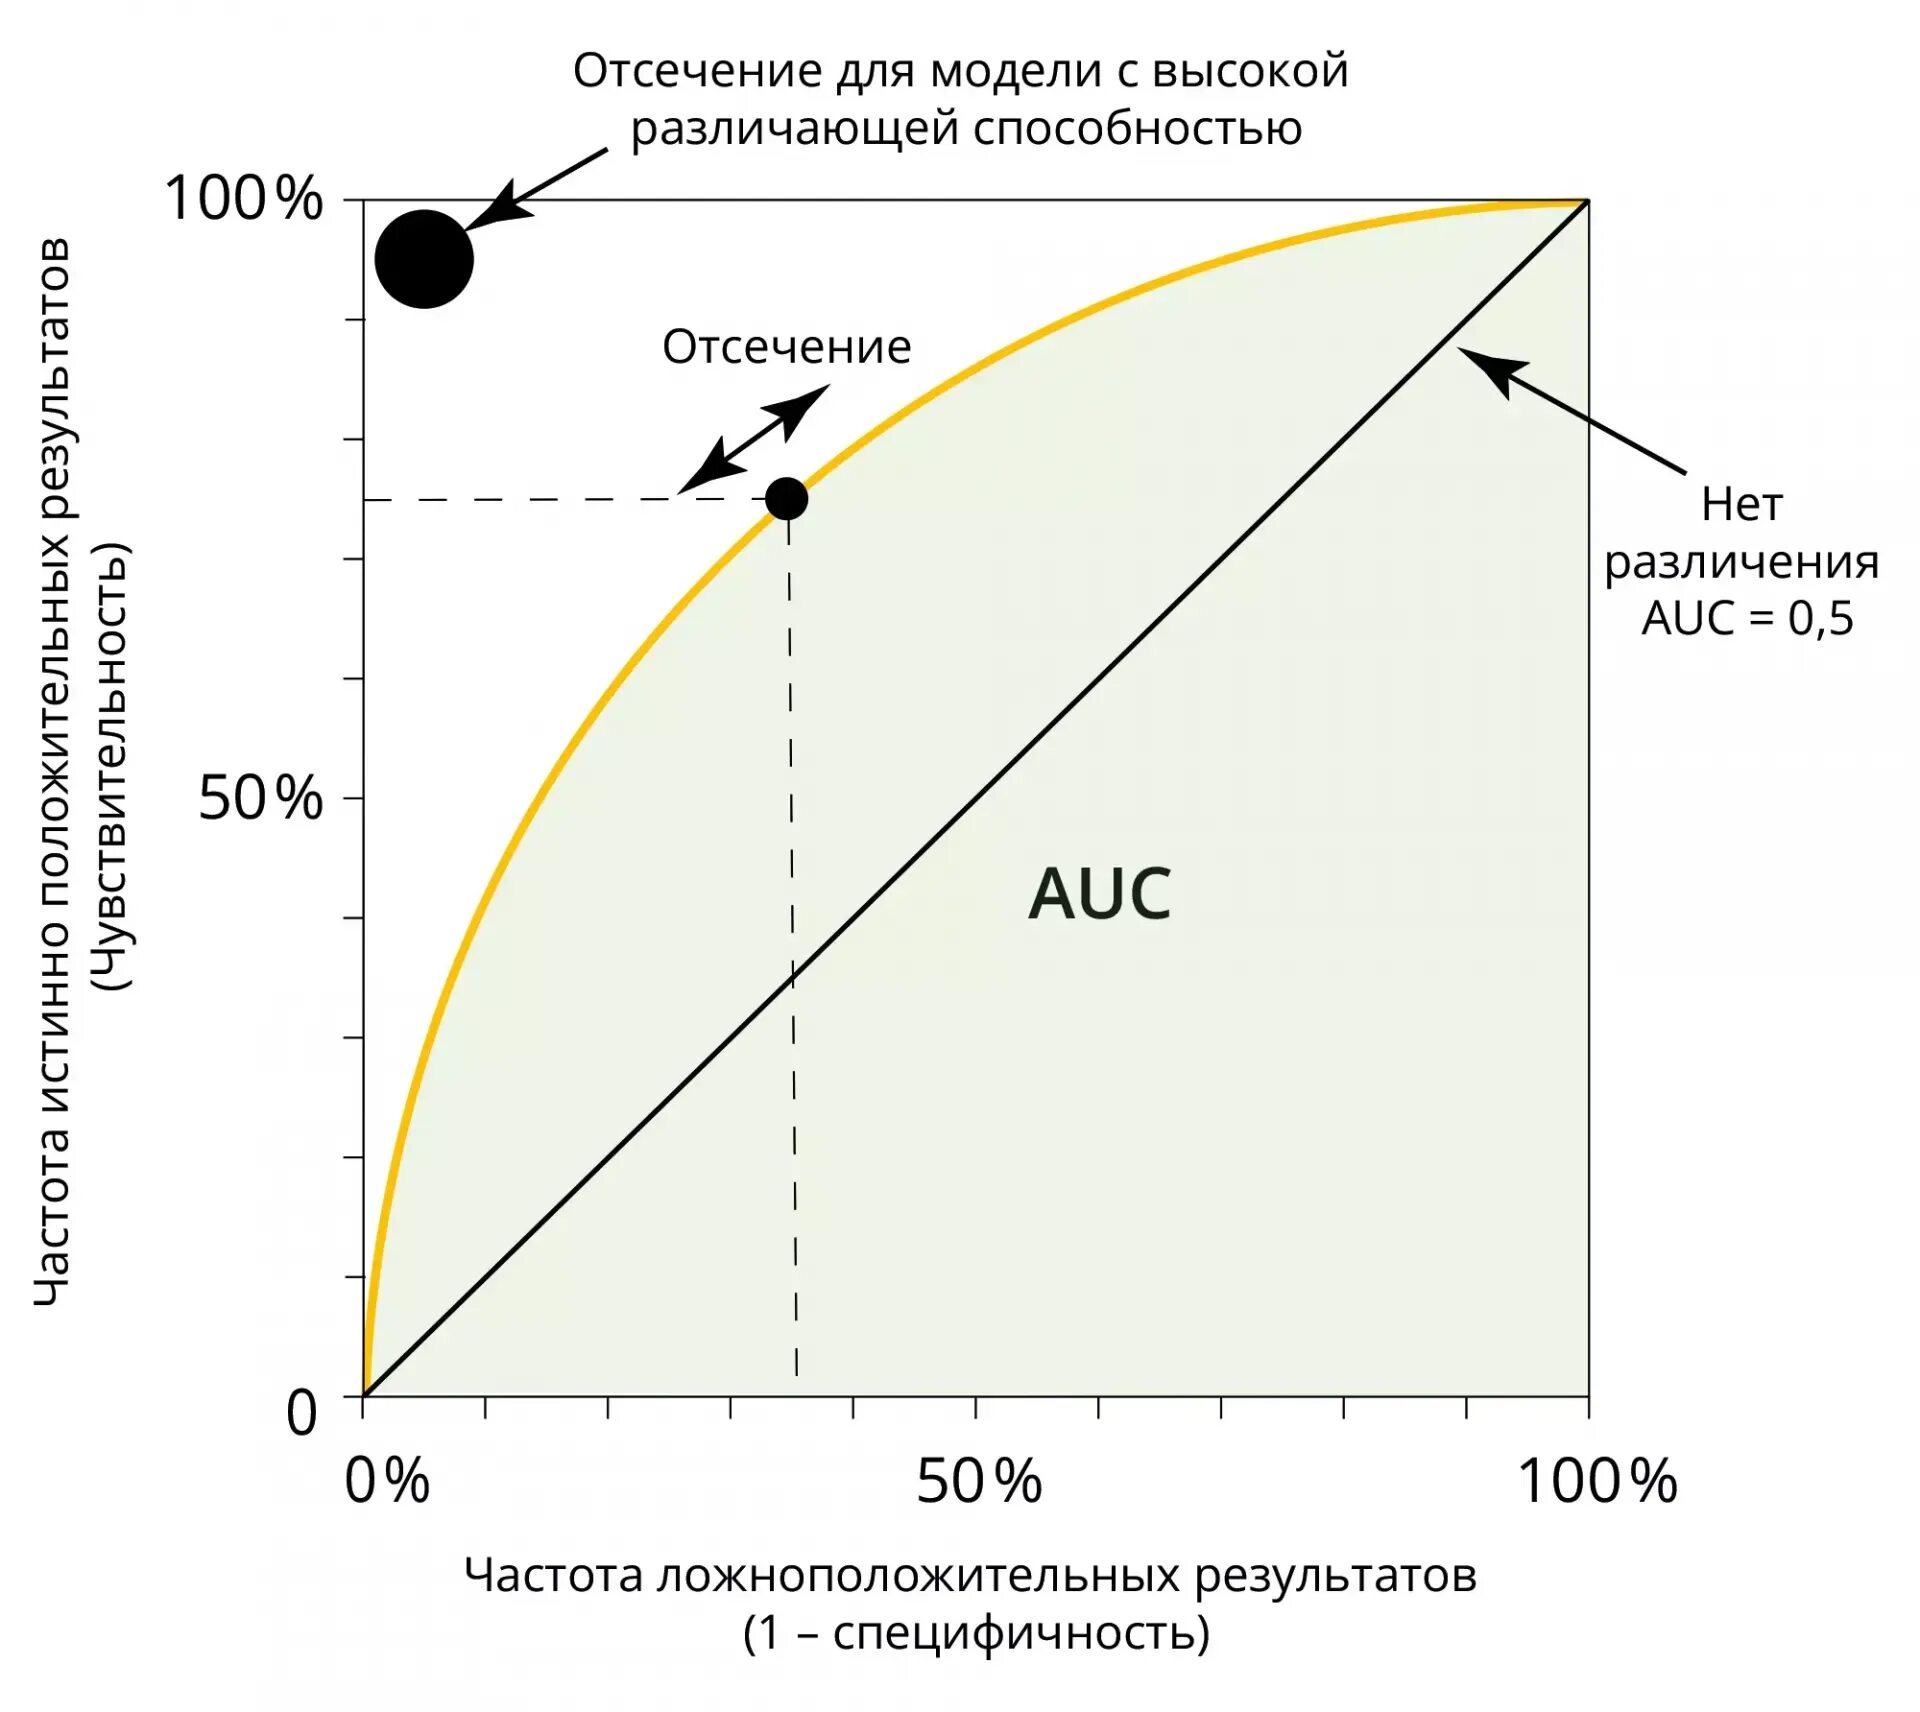
\includegraphics[width=0.66\textwidth]{ml_metric_roc.jpeg}
    \caption{ROC-кривая и изменение рабочей точки при выборе порога.
    Иллюстрация из исследования архитектур нейросетей}
    \label{fig:ch4_metric_roc}
\end{figure}

Высокая ROC-AUC сама по себе не определяет подходящую уставку
и не показывает частоту ложных сообщений в эксплуатации.
Для выбранного порога используются Precision и Recall,
рассматриваемые совместно с составом проверочных режимов. При нескольких метках
показатели сначала определяются для каждого события.
Усреднение по классам с одинаковым весом и объединение всех
решений в общий подсчёт отвечают на разные вопросы.
В дальнейшем эти варианты различаются как усреднение
по классам и подсчёт по совокупности решений.

\subsection{Единица оценки и независимая проверка}
\label{sec:ch4_metric_validation}

Временная метка, окно, интервал события и целая осциллограмма
являются разными единицами оценки. Один правильно найденный
участок может быть достаточен для обнаружения события в записи,
но не означает правильного восстановления всех его границ.
Аналогично большое число соседних окон не превращает одну
осциллограмму в множество независимых испытаний.
В дальнейшем отдельно рассматриваются классификация окна,
разметка последовательности и обнаружение события в записи.

Обучающая выборка используется для настройки параметров сети,
валидационная для выбора конфигурации и состояния модели,
а проверочная для оценки выбранного решения. Эти назначения
различаются при описании состава данных и порядка разделения
записей. Если используются синтетические
режимы и реальные осциллограммы, результаты по ним приводятся
отдельно. Специально отобранные сложные неаварийные процессы
позволяют исследовать характер ошибок, но их доля не задаёт
частоту ложных действий на полном потоке.

Для РНМ положительной меткой становится требуемое состояние
выхода органа в применимом режиме. При этом направление,
условия применимости и интервалы переходного процесса
определяются собственной разметкой. Проверка такого выхода
рассматривается в главе~\ref{ch:ml_adaptive_algorithms}
с использованием приведённых здесь определений.

\subsection{Вычислительная сложность и быстродействие}
\label{sec:ch4_metric_runtime}

Число обучаемых параметров характеризует размер модели,
но не определяет время её расчёта. Сложность операций,
подготовка признаков и реализация слоёв могут существенно
различаться. В архитектурном исследовании рассматриваются два отдельных
сопоставления качества, по числу параметров и по времени расчёта
одного окна на CPU. Они характеризуют размер обучаемой части
и вычислительные затраты использованной программной реализации.
Такое сравнение не является измерением времени действия
готового терминала БАВР.

Для БАВР существенно время получения решения после изменения
режима. Оно зависит от необходимой предыстории, шага обработки
и устойчивости выхода во времени наряду с временем вычислений.
В настоящей главе время расчёта окна рассматривается отдельно
от задержки обнаружения события. Переход к времени действия
органа связан с последующими предметными испытаниями.

\iffalse
(Примечание автора: Вот не надо писать так обще для будущих пользователей метрик, говори что в используется, рассматривается, а не «вы должны», или не пиши такое вообще, как тут, так и в других местах, устал повторять об этом.) **[AA066: закрыто автором; сохранено в истории]**
(Примечание автора: Можно считать закрытой и убирать отсюда, прост не забудь в своих инструкциях на будущее, чтобы не допускать такие косяки, как и по другим комментариям)
\fi
\authorreviewnote{AA066}

\iffalse
(Примечание автора: И вот тут «должно сопровождаться», пишется как инструкция для других, а не то, что используется в диссертации… в общем, вот эти моменты требуют правок, дальше не буду даже отмечать это, глянь прост.) **[AA067: закрыто автором; сохранено в истории]**
(Примечание автора: Аналогично, можно считать закрытой и убирать)
\fi
\authorreviewnote{AA067}

\iffalse
(Примечание автора: На будущее пометка – а разве у меня вообще где-то это указывается в исследованиях? Может вот это стоит пометить как «требуется разделять по аппаратной части, сложности вычислений и т.д., а мы смотрим тут вот это?». Это пока вопрос, может в статьях у нас и норм, прост не уверен.) **[AA068: закрыто автором; сохранено в истории]**
(Примечание автора: Ок, создай задачу на будущее, может сделаем, может нет, она не обязательна, может будет указано / учтено только местами, где есть, ибо перезапускать всё точно не буду, так что она желательна, если есть информация или ещё не сложно запустить опыты, но не обязательна. И сейчас может считаться закрытой.)
\fi
\authorreviewnote{AA068}
